\chapter{Theoretical Motivation} \label{chap-theory}

DGLAP
Higgs related to top
interaction lagrangian with effective operators
electric dipole moment and a top quark with 4/3 charge
anomolous couplings
talk about top quarks - different chapter maybe?

\begin{figure}
\begin{center}
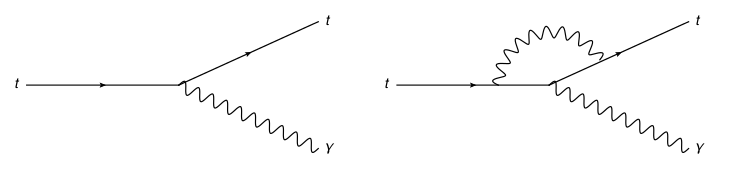
\includegraphics[width=\textwidth]{Figures/TopPhotonVertex.png}
\caption{Top-photon vertex. Left: Leading Order (LO). Right: One-Loop correction (NLO).}
\end{center}
\end{figure}

\begin{equation} \label{eqn-interactionlagrangian}
\lumi_{t\bar{t}\gamma} = -eQ_t\bar{t}\gamma^{\mu}tA_{\mu} - e\bar{t}\frac{i\sigma^{\mu\nu}q_{\nu}}{m_t}(d^{\gamma}_V+id^{\gamma}_A\gamma^5)tA_{\mu}
\end{equation}

\begin{align}\label{eqn-smparameterisations}
\delta d^{\gamma}_V = \frac{\sqrt{2}}{e}\text{Re}[c_WC^{33}_{uB\phi} + s_WC^{33}_{uW}]\frac{vm_t}{\Lamdba^2} \\
\delta d^{\gamma}_A = \frac{\sqrt{2}}{e}\text{Im}[c_WC^{33}_{uB\phi} + s_WC^{33}_{uW}]\frac{vm_t}{\Lamdba^2}
\end{align}